%! TEX root = **/report.tex
\section{Analyzing and building our own network}

\subsection{Generating our network}

\subsubsection{Data sources}

For our own network, we decided to use the \emph{arXiv} abstract documents we have already
worked with in previous sessions. The dataset consists of abstracts of scientific papers
from the \emph{arXiv} repository.

To build the network, we decided to use TF-IDF and cosine similarity to decide which
nodes to add. Similarly to what we did in laboratory session 2, where we used
cosine similarity and TF-IDF to find the most similar papers for a given document.

That is, we wanted to compute the pairwise cosine similarity between all documents in the
collection. However, this is computationally expensive, given that we have around 55,000 documents.

\begin{figure}[H]
	\begin{tikzpicture}
		[node/.style={draw, minimum height=1cm}]
		% diagram of steps to build network
		\node[node] (data) {arXiv abstracts};
		\node[node, below = of data] (tfidf) {TF-IDF matrix};
		\node[node, below = of tfidf] (sim) {Cosine similarity matrix};
		\node[node, below =of sim] (net) {Adjacency list};
		\node[node, below = of net] (graph) {\texttt{networkx} graph};

		\path[->] (data) edge node[right] {\texttt{sklearn.feature\_extraction.text.TfidfVectorizer}} (tfidf);
		\path[->] (tfidf) edge node[right] {\texttt{sklearn.metric.pairwise.cosine\_similarity}} (sim);
		\path[->] (sim) edge node[right] {\texttt{np.flatnonzero(d < threshold)}} (net);
		\path[->] (net) edge node[right] {\texttt{networkx.from\_edgelist}} (graph);
	\end{tikzpicture}
	\caption{Diagram of the steps to build the network.}
\end{figure}

\subsubsection{Computational challenges}

Computing the TF-IDF matrix is feasible, given that it is a sparse matrix. We can use
the \texttt{sklearn.feature\_extraction.text.TfidfVectorizer} class to compute the TF-IDF
matrix. This is much faster than any other python implementation we could have developed by ourselves
and builds the matrix in a \emph{numpy} sparse matrix in less than 30 seconds.

\begin{minted}{python}
import pathlib
from sklearn.feature_extraction.text import TfidfVectorizer

folder = pathlib.Path("data/arxiv_abs")
files = filter(lambda x: x.is_file(), pathlib.Path(folder).glob("**/*"))

vectorizer = TfidfVectorizer(input="filename")
X = vectorizer.fit_transform(files)
\end{minted}

Once we have the TF-IDF matrix, we can try to compute the pairwise cosine similarity, but
we soon realize that it is not feasible. With 55.000 documents and using 64-bit floats, the
matrix would require 24Gb of memory. We know that the matrix is symmetric and that we only
need to compute the upper triangular part of the matrix, however the memory requirements
are still too high for our computers to do any computations on top of it.

From this point, we had to options: sub-sample the dataset or find a way to compute the
data in batches that can fit into memory.

Since our final goal is to build a network, we don't really care about the exact value of the
cosine similarity, but rather about whether or not two documents are similar enough to be
connected. Therefore, we can compute the cosine similarity in batches and reduce it by keeping
only the indices of the documents that are similar within a given threshold.

Fortunately, \texttt{sklearn} provides a method to compute distances in batches and reduce it
with a custom method. We can use the \texttt{sklearn.metrics.pairwise\_distances\_chunked}
along with our custom reducer that extracts only the indices of the documents that are
withing our wanted threshold:

\begin{minted}{python}
from sklearn.metrics import pairwise_distances_chunked
from itertools import chain

threshold = 0.7

def reduce_func(D_chunk, start):
     # we use cosine distance, not similarity (distance = 1 - similarity)
     # therfore, we use < instead of >
     return [np.flatnonzero(d < threshold) for d in D_chunk]

gen = pairwise_distances_chunked(X, metric="cosine", working_memory=None, reduce_func=reduce_func)

adjacency_list = list(chain.from_iterable(gen))
\end{minted}

The only issue is that if we want to change the threshold, we have to recompute
the pairwise distances again. However, the computation is fast enough (around 7 minutes)
that we can afford to do it.

\subsection{Analysis}

The TF-IDF matrix had 55760 documents and 108408 unique words. From that, using a threshold
of distance at most 0.7 (similarity of more than 0.3), we obtained a network
with 50\,245 nodes and 427\,112 edges.
Some nodes had no connections, so they were removed from the network, that is why there
are fewer nodes than documents.

Additionally, we are only interested in the largest connected component of the network, so we
need to find the largest connected component and remove the rest of the nodes and edges. After
this step, we are left with 43\,665 nodes and 420\,662 edges.

\subsubsection{Metrics}

The network has a diameter%
\footnote{Using \texttt{networkx.approximate.diameter}, since the exact diameter is too expensive to compute for our graph.}
of 21 and a transitivity of 0.3687.

The degree distribution of the network is shown in Figure~\ref{fig:degree_dist}. We can see that
the distribution is skewed to the right. Most nodes have a degree between 1 and 100. There are
a couple of nodes with very high degree.

\begin{figure}[H]
	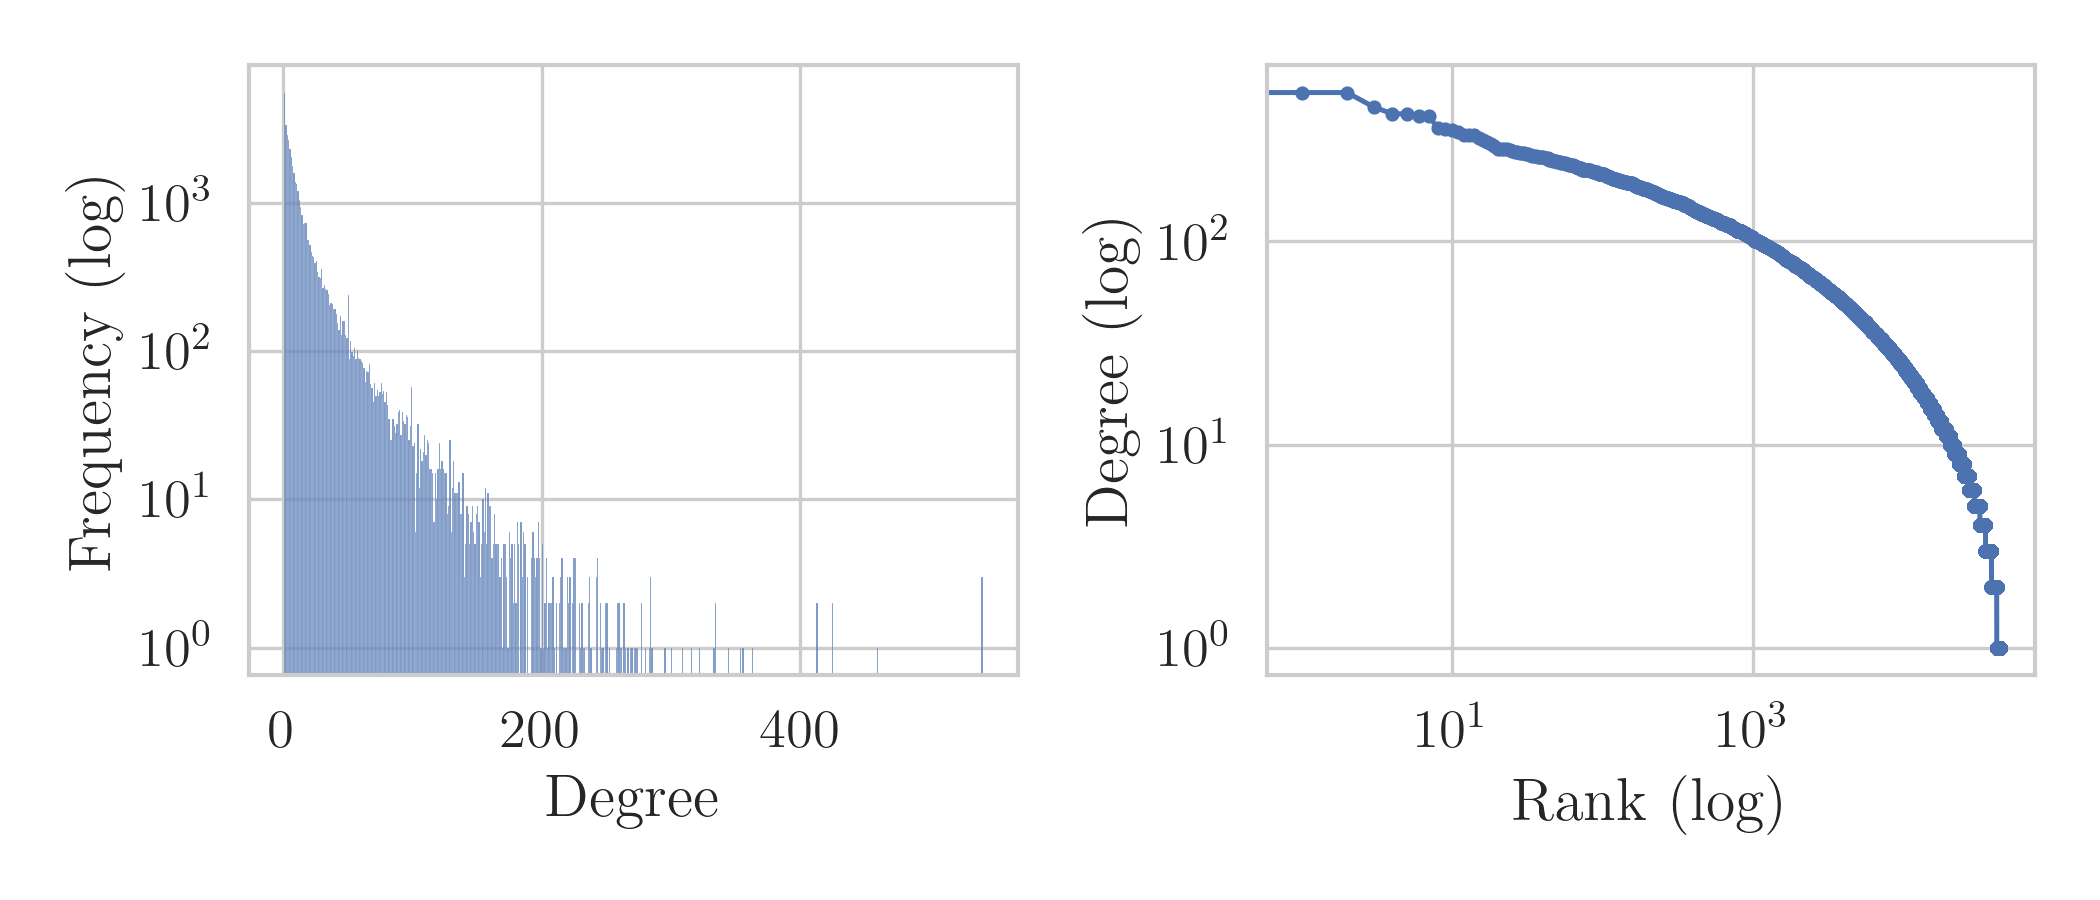
\includegraphics{figures/degree_joint.png}
	\caption{Degree distribution and rank-degree plot of the network.}%
	\label{fig:degree_dist}
\end{figure}

A priori, it may seem like a \emph{Barabasi-Albert} model, but if we plot the log-log of the
degree distribution as we did in the previous section for the \emph{BA} model, we can
see that it is not the case. This is shown in \cref{fig:degree_dist_fit}, where it is clear
that the \emph{BA} model does not fit the data.

\begin{figure}[H]
    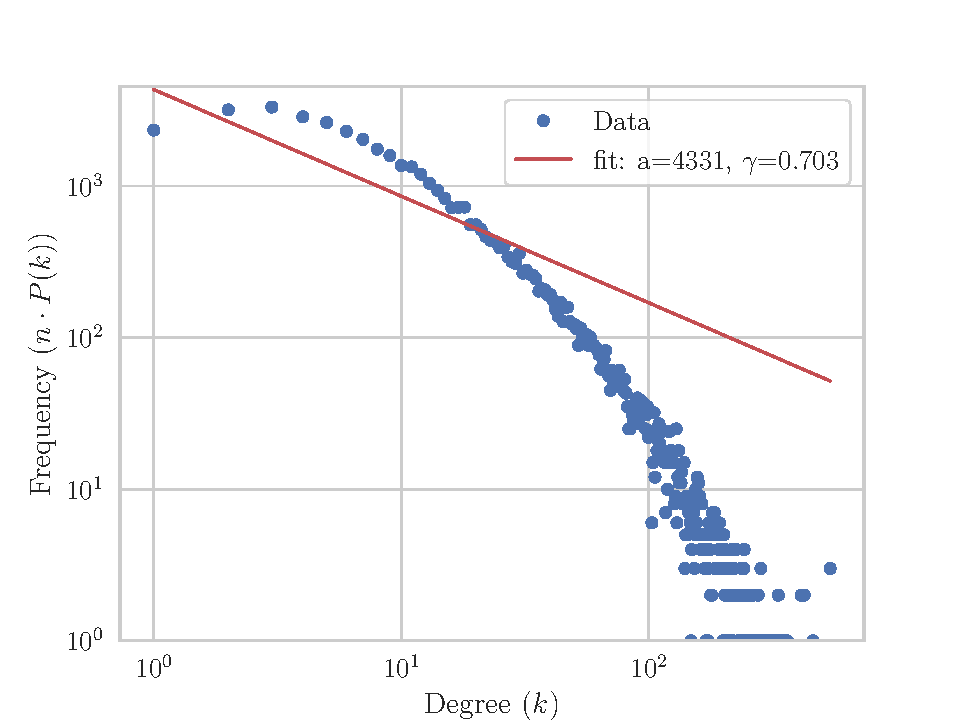
\includegraphics{figures/ba_fit_2nd}
    \caption{Log-log plot of the degree distribution of the network.}%
    \label{fig:degree_dist_fit}
\end{figure}

\pagebreak
\subsubsection{PageRank}

The results of applying the \emph{PageRank} algorithm to the network are shown in
\cref{tab:pagerank}.

\begin{table}[H]
	\caption{Top 10 nodes with highest PageRank.}%
    \label{tab:pagerank}
	\begin{tabular}{lrr}
		\toprule
		Category & Doc ID & PageRank   \\
		\midrule
		astro-ph & 002039 & 0.00047309 \\
		astro-ph & 010564 & 0.00034578 \\
		math     & 000270 & 0.00034277 \\
		astro-ph & 000188 & 0.00033910 \\
		hep-th   & 000005 & 0.00033910 \\
		astro-ph & 010648 & 0.00033449 \\
		cs       & 015444 & 0.00032901 \\
		math     & 006008 & 0.00032901 \\
		quant-ph & 001595 & 0.00032901 \\
		cs       & 010628 & 0.00027116 \\
		\bottomrule
	\end{tabular}
\end{table}

We can see that of the top 10 nodes, 4 are from the \emph{astro-ph} category. If we look at the
sizes of each category, we can see that \emph{astro-ph} is the largest category, so it is not
surprising that it has the most important nodes. Also, we can see that in the top 10, there are some
nodes with the exact same \emph{PageRank} value. Upon further inspection, we found that these were in
fact the same abstract which was duplicated in different categories. This duplication may have inflated
the \emph{PageRank} of the nodes.

Unfortunately, we were not able to obtain a proper visualization of the PageRank network, since
the network was too large. Maybe using another visualization tool instead of the one provided by
\texttt{networkx} would have helped in that regard.

\pagebreak
\subsubsection{Communities}

We applied the Louvain algorithm to the network to find communities. We used the
\texttt{networkx} implementation. The algorithm was able to find
74 communities. The biggest community has 2\,750 nodes and the smallest has
only 5 nodes. The size distribution of the communities is shown in Figure~\ref{fig:communities}.

\begin{figure}[H]
	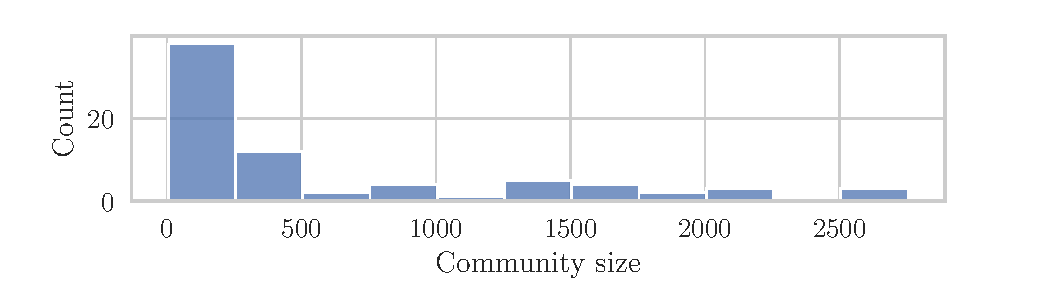
\includegraphics{figures/community_dist.pdf}
	\caption{Size distribution of the communities.}%
	\label{fig:communities}
\end{figure}

Most of the communities had small sizes, but there is a fair amount of communities with
more than 500 nodes. The \emph{arXiv} abstracts that we used came from 8 different categories,
so we have almost 10 times more communities than original categories. This may indicate
that we are finding communities that correspond to sub-categories of the original 8.

If we take a look at the biggest community, as shown in Figure~\ref{fig:big_community}, we can see
that it is mostly composed of papers from the \emph{astro-ph} category and is very
densely connected.

\begin{figure}[H]
	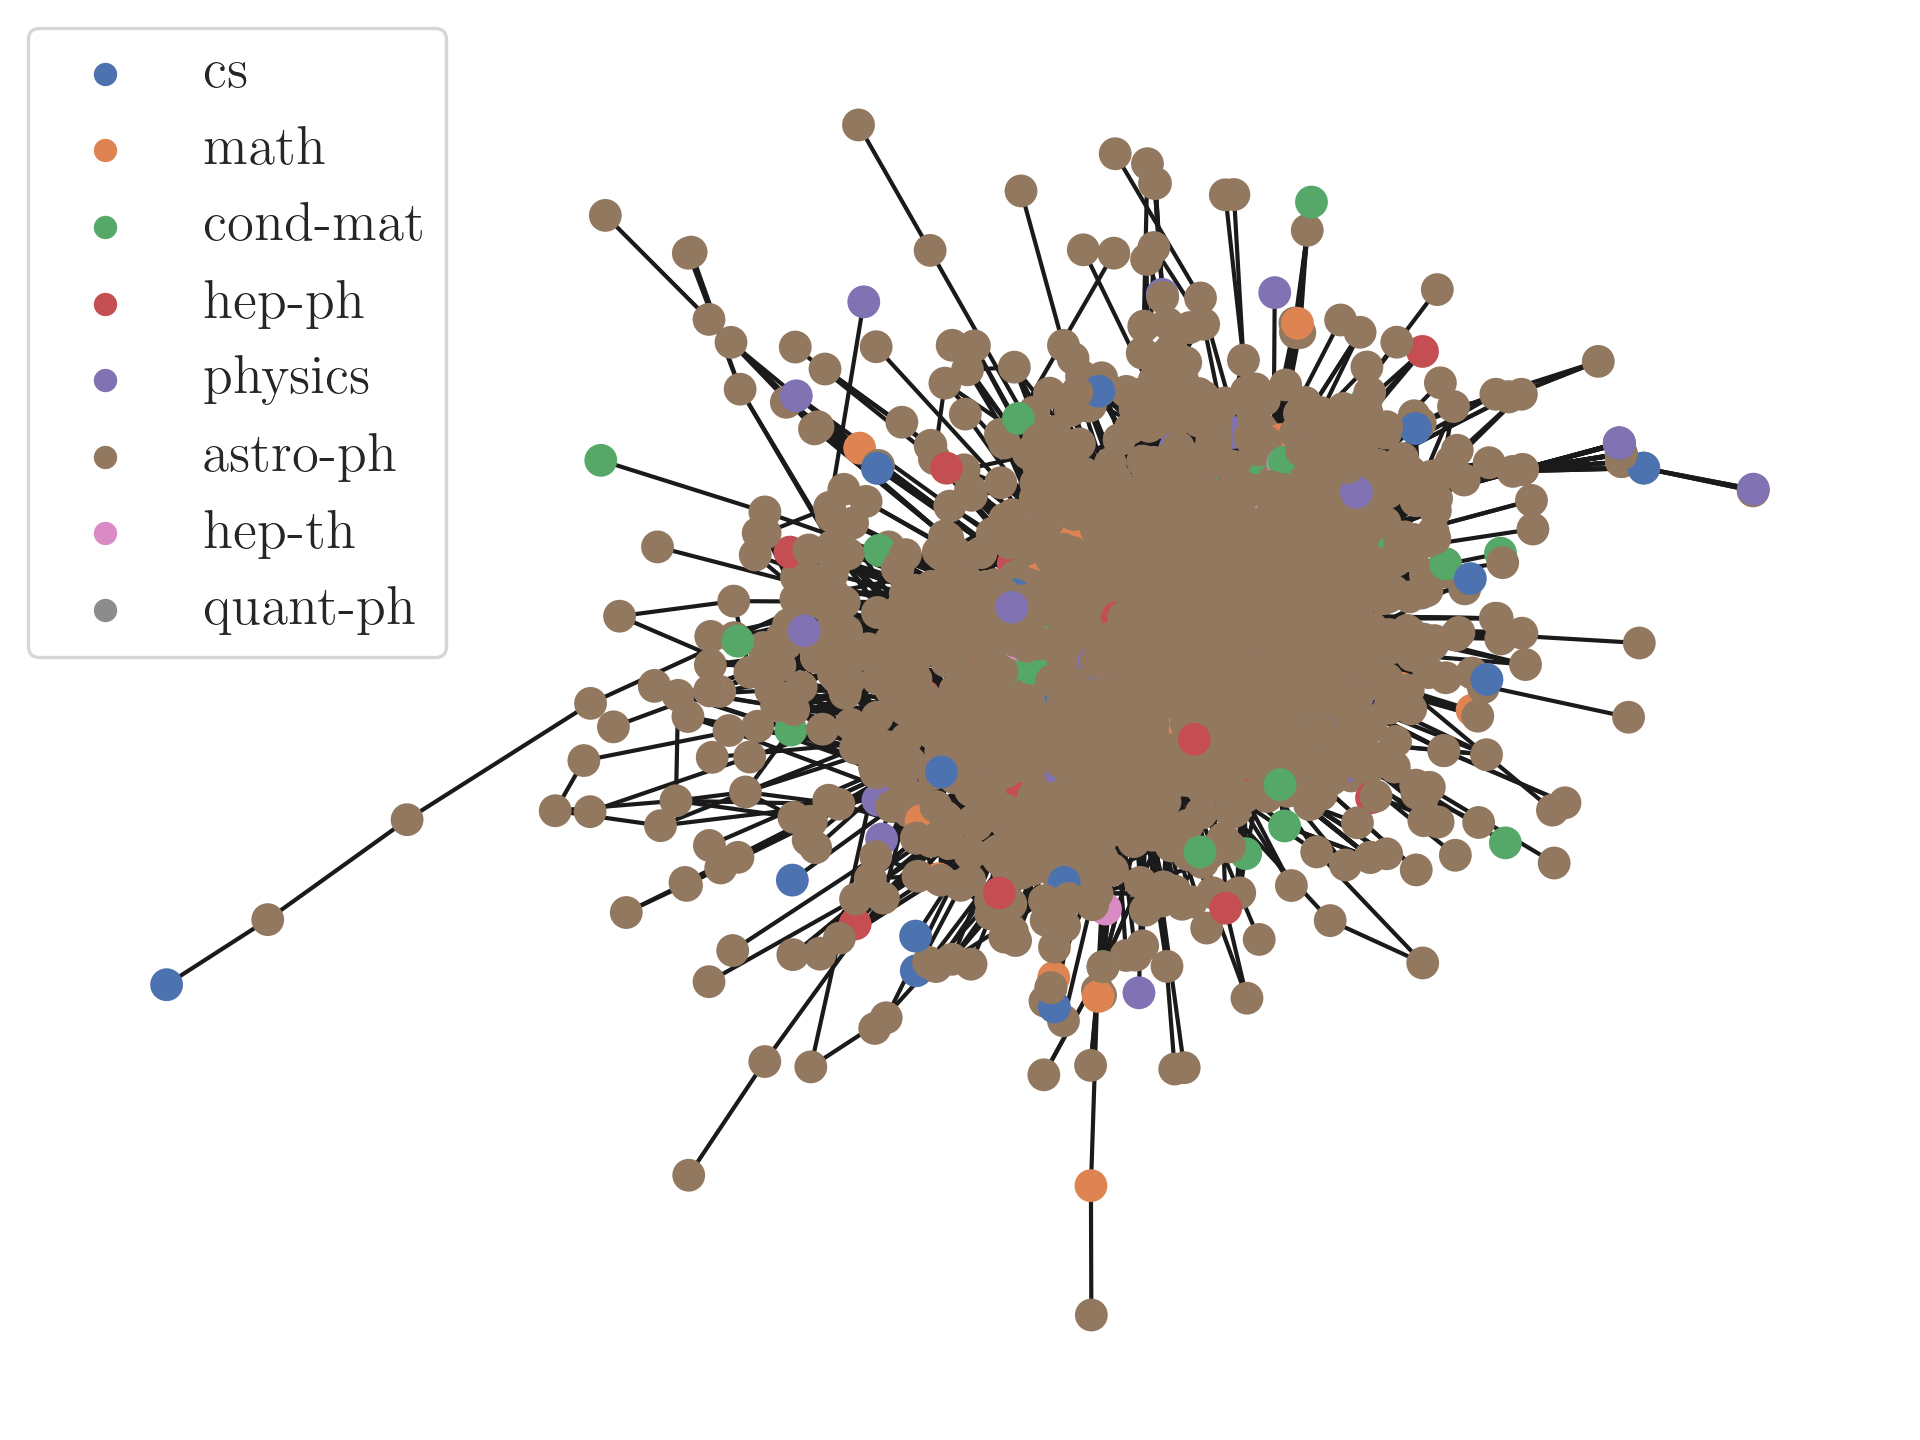
\includegraphics{figures/community.png}
	\caption{The biggest community of the network.}%
	\label{fig:big_community}
\end{figure}

Looking at other communities and computing the frequency of each of the categories,
we can see that there is always a clear dominant category in the
bigger communities. \Cref{fig:community_freq} shows
the distribution of the categories inside the community with most nodes shown in
the graph of \cref{fig:big_community}. \Cref{fig:community_freq_cs} shows the frequency of
another community that is mostly composed of papers from the \emph{cs} category but also
a significant amount of papers from the \emph{math} category. This overlap of math and computer
science is not surprising given that we are using TF-IDF and many papers will use similar
terminology and concepts in these categories.

% \pagebreak\null
\begin{multicols}{2}
	\begin{figure}[H]
		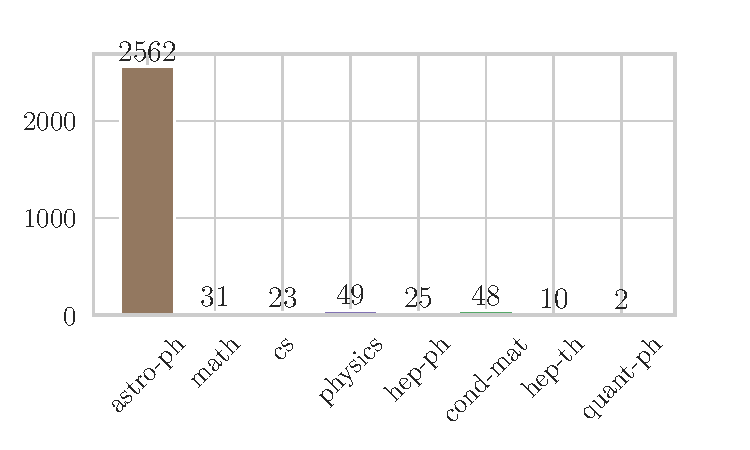
\includegraphics[width=0.49\textwidth]{figures/community_dist_biggest}
		\caption{Frequency of the categories in the communities of the biggest community}%
		\label{fig:community_freq}
	\end{figure}

	\begin{figure}[H]
		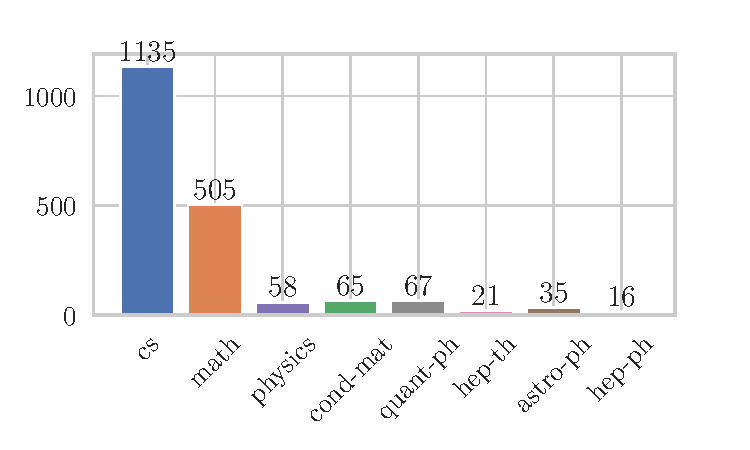
\includegraphics[width=0.49\textwidth]{figures/community_dist_cs}
		\caption{Frequency of the categories in the communities of community 40}%
		\label{fig:community_freq_cs}
	\end{figure}
\end{multicols}
